\begin{tabular}{M{6.5cm}M{11cm}}
	\textbf{TRUNG TÂM MANABIE}& \textbf{ĐỀ ÔN TẬP KIỂM TRA GIỮA HỌC KÌ 1}\\
	\textbf{MÃ ĐỀ: 003}& \textbf{Bài thi môn: VẬT LÝ 12}\\
	\textit{(Đề trường TH - THCS - THPT\newline Lê Thánh Tông năm 2024 -2025)}& \textit{Thời gian làm bài: 50 phút, không kể thời gian phát đề}
	
	\noindent\rule{4cm}{0.8pt} \\
\end{tabular}
\setcounter{section}{0}
\section{Câu trắc nghiệm nhiều phương án lựa chọn}
\textit{Thí sinh trả lời từ câu 1 đến câu 18. Mỗi câu hỏi thí sinh chọn một phương án}
\setcounter{ex}{0}
\Opensolutionfile{ans}[ans/G12-3-TN]
% ===================================================================
\begin{ex}
	Nhiệt lượng mà một vật đồng chất thu vào để tăng nhiệt độ thêm $\SI{40}{\celsius}$ là $\SI{17.6}{\kilo\joule}$. Bỏ qua sự trao đổi nhiệt với môi trường. Biết khối lượng của vật là $\SI{500}{\gram}$, nhiệt dung riêng của chất làm vật là	
	\choice
	{$\SI{112.5}{\joule/\kilogram\cdot\kelvin}$}
	{$\SI{460}{\joule/\kilogram\cdot\kelvin}$}
	{$\SI{380}{\joule/\kilogram\cdot\kelvin}$}
	{\True $\SI{880}{\joule/\kilogram\cdot\kelvin}$}
	\loigiai{$c=\dfrac{Q}{m\Delta t}=\SI{880}{\joule/\kilogram\cdot\kelvin}$}
\end{ex}
% ===================================================================
\begin{ex}
	Trường hợp nào dưới đây làm biến đổi nội năng của vật không phải do thực hiện công?
	\choice
	{Khuấy nước}
	{Mài dao}
	{\True Nung đồng trong lò}
	{Đóng đinh}
	\loigiai{}
\end{ex}
% ===================================================================
\begin{ex}
	Chọn phát biểu đúng về sự nóng chảy của một chất nào đó.
	\choice
	{\True Cần cung cấp nhiệt lượng}
	{Xảy ra ở cùng nhiệt độ với sự hoá hơi}
	{Xảy ra ở $\SI{100}{\celsius}$}
	{Toả nhiệt ra môi trường}
	\loigiai{}
\end{ex}
% ===================================================================
\begin{ex}
	Một thước $\si{\centi\meter}$ được đặt dọc theo một nhiệt kế thủy ngân chưa được chia vạch như hình dưới đây. Trên nhiệt kế chỉ đánh dấu điểm đóng băng và điểm sôi của nước tinh khiết ở áp suất tiêu chuẩn. Giá trị nhiệt độ đang hiển thị trên nhiệt kế là bao nhiêu?
	\begin{center}
		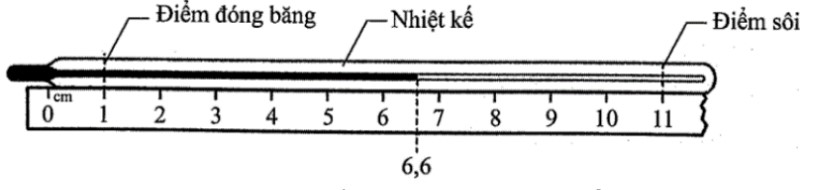
\includegraphics[width=0.5\linewidth]{../figs/D12-2-1}
	\end{center}
	\choice
	{\True $\SI{56}{\celsius}$}
	{$\SI{60}{\celsius}$}
	{$\SI{66}{\celsius}$}
	{$\SI{44}{\celsius}$}
	\loigiai{
		$\dfrac{t-t_b}{t_s-t_b}=\dfrac{\ell-\ell_b}{\ell_s-\ell_b}\Leftrightarrow \dfrac{t-0}{100-0}=\dfrac{6,6-1}{11-1}\Rightarrow t=\SI{56}{\celsius}.$
	}
\end{ex}
% ===================================================================
\begin{ex}
	Một căn phòng có thể tích $\SI{50}{\meter^3}$. Khi tăng nhiệt độ của phòng từ $\SI{20}{\celsius}$ đến $\SI{30}{\celsius}$ thì khối lượng không khí (coi là khí lí tưởng) thoát ra khỏi căn phòng là bao nhiêu kilogram? Coi áp suất khí trong phòng không đổi. Biết khối lượng riêng của không khí ở $\SI{20}{\celsius}$ là $\SI{1.2}{\kilogram/\meter^3}$.	
	\choice
	{\True $\SI{1.98}{\kilogram}$}
	{$\SI{30.00}{\kilogram}$}
	{$\SI{2.05}{\kilogram}$}
	{$\SI{1.98}{\kilogram}$}
	\loigiai{
		Trong điều kiện áp suất không đổi:
		$$\dfrac{D_2}{D_1}=\dfrac{V_1}{V_2}=\dfrac{T_1}{T_2}\Rightarrow D_2\approx\SI{1.16}{\kilogram/\meter^3}$$
		Khối lượng không khí thoát ra khỏi căn phòng:
		$$\Delta m=m_1-m_2=\left(D_1-D_2\right)V=\SI{1.98}{\kilogram}.$$
	}
\end{ex}
% ===================================================================
\begin{ex}
	\immini{
		Hình bên là đồ thị biểu diễn sự phụ thuộc của áp suất $p$ theo thể tích $V$ khi nhiệt độ không đổi của một lượng khí lí tưởng xác định. Gọi $S_{1}$ và $S_{2}$ lần lượt là diện tích của các hình chữ nhật ABCD và DEFG. Hệ thức đúng giữa $S_{1}$ và $S_{2}$ là
		\choice
		{$S_{1}>S_{2}$}
		{$3 S_{1}=2 S_{2}$}
		{$S_{1}<S_{2}$}
		{\True $S_{1}=S_{2}$}
	}
	{
		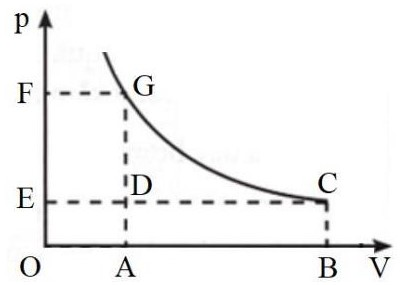
\includegraphics[width=0.5\linewidth]{../figs/D12-2-2}
	}
	\loigiai{
		Quá trình biến đổi từ G$\rightarrow$ C là đẳng nhiệt nên $p_{\mathrm{G}}V_{\mathrm{G}}=p_{\mathrm{C}}V_{\mathrm{C}}\Rightarrow S_{\mathrm{BCEO}}=S_{\mathrm{AGFO}}\Rightarrow S_{\mathrm{ABCD}}=S_{\mathrm{EFGD}}$.
	}
\end{ex}
% ===================================================================
\begin{ex}
	Trong một quá trình biến đổi, nội năng của một khối khí giảm đi $\SI{15}{\joule}$. Nếu trong quá trình đó khối khí nhận vào một nhiệt lượng là $\SI{35}{\joule}$ thì khối khí đã 
	\choice
	{sinh công $\SI{20}{\joule}$}
	{nhận công $\SI{50}{\joule}$}
	{nhận công $\SI{20}{\joule}$}
	{\True sinh công $\SI{50}{\joule}$}
	\loigiai{
		$\Delta U=Q+A\Rightarrow A=\Delta U-Q=-15-35=\SI{-50}{\joule}.$
	}
\end{ex}
% ===================================================================
\begin{ex}
	\immini{
		Một khối khí lí tưởng xác định biến đổi theo các quá trình (1) - (2) - (3) - (4) như hình vẽ. Cho $p$ là áp suất và $V$ là thể tích của khối khí. Biết nhiệt độ của khối khí ở trạng thái (4) là $\SI{-153}{\celsius}$. Nhiệt độ của khối khí này ở trạng thái (1) là
		\choice
		{$\SI{960}{\celsius}$}
		{\True $\SI{687}{\celsius}$}
		{$\SI{1224}{\celsius}$}
		{$\SI{1233}{\celsius}$}
		
	}
	{
		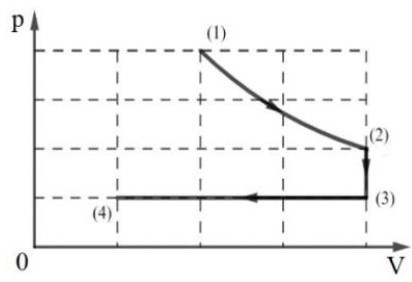
\includegraphics[width=0.55\linewidth]{../figs/D12-2-3}
	}
	\loigiai{
		$$\dfrac{p_1V_1}{T_1}=\dfrac{p_4V_4}{T_4}\Leftrightarrow \dfrac{4\cdot2}{T_1}=\dfrac{1\cdot1}{-153+273}\Rightarrow T_1=\SI{960}{\kelvin}\Rightarrow t_1=\SI{687}{\celsius}.$$
	}
\end{ex}

% ===================================================================
\begin{ex}
	Một ống thủy tinh tiết diện đều một đầu kín, một đầu hở, chiều dài $L=\SI{50}{\centi\meter}$, có một cột thủy ngân dài $H =\SI{19}{\centi\meter}$ bịt kín một cột không khí trong ống. Coi nhiệt độ không đổi. Khi đặt ống thủy tinh nằm ngang thì chiều dài cột không khí là $L_1=\SI{20}{\centi\meter}$. Khi đặt ống thủy tinh thẳng đứng với đầu hở ở trên thì chiều dài cột không khí là $L_2=\SI{16}{\centi\meter}$. Nếu ống thủy tinh được đặt thẳng đứng với đầu hở ở dưới thì chiều dài của cột không khí bên trong ống là
	\choice
	{$\SI{22.12}{\centi\meter}$}
	{$\SI{50.00}{\centi\meter}$}
	{$\SI{25.73}{\centi\meter}$}
	{$\SI{26.67}{\centi\meter}$}
	\loigiai{
		$$p_0L_1=\left(p_0+H\right)L_2=\left(p_0-H\right)L_3\Rightarrow \begin{cases}
			p_0=\SI{76}{\centi\meter Hg}\\
			L_3\approx\SI{26.67}{\centi\meter}
		\end{cases}.$$
	}
\end{ex}
% ===================================================================
\begin{ex}
	Hàn thiếc là một phương pháp nối kim loại với nhau bằng một kim loại hay hợp kim trung gian (thiếc) gọi là vảy hàn. Trong quá trình nung nóng để hàn, vảy hàn sẽ nóng chảy trước trong khi vật hàn chưa nóng chảy hoặc nóng chảy với số lượng không đáng kể. Khi đó kim loại làm vảy hàn sẽ khuếch tán thẩm thấu vào trong kim loại vật hàn tạo thành mối hàn. Thiếc hàn là hợp kim	thiếc - chì có nồng độ phù hợp với mục đích sử dụng. Ví dụ thiếc hàn 60 ($\SI{60}{\percent}\ \ce{Sn}$ và $\SI{40}{\percent}
	\ \ce{Pb}$) được sử dụng để hàn các dây dẫn hay mối nối trong mạch điện. Thiếc hàn phải có
	\choice
	{nhiệt độ nóng chảy và nhiệt nóng chảy riêng lớn hơn của kim loại vật hàn}
	{nhiệt độ nóng chảy lớn để tránh nóng chảy mối hàn trong quá trình sử dụng}
	{\True nhiệt độ nóng chảy và nhiệt nóng chảy riêng nhỏ hơn của kim loại vật hàn}
	{nhiệt nóng chảy riêng lớn để tránh nóng chảy mối hàn trong quá trình sử dụng}
	\loigiai{
		Vảy hàn phải có nhiệt độ nóng chảy và nhiệt dung riêng nhỏ hơn vật hàn để nóng chảy trước.
	}
\end{ex}
% ===================================================================
\begin{ex}
	Cho $p$ là áp suất, $V$ là thể tích, $T$ là nhiệt độ tuyệt đối của một lượng khí lí tưởng xác định. Hình nào dưới đây biểu diễn quá trình biến đổi trạng thái của lượng khí đó khác với các hình còn lại?
	\begin{center}
		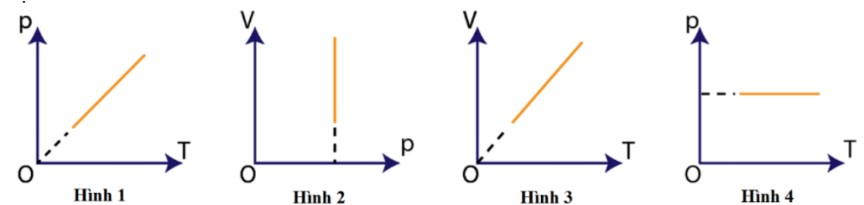
\includegraphics[width=0.7\linewidth]{../figs/D12-2-4}
	\end{center}
	\choice
	{Hình 3}
	{Hình 4}
	{Hình 2}
	{\True Hình 1}
	\loigiai{
		Hình 1 là quá trình đẳng tích, các hình còn lại là quá trình đẳng áp.
	}
\end{ex}
% ===================================================================
\begin{ex}
	Trong thí nghiệm kiểm chứng lại định luật Boyle, việc dịch chuyển pit-tông từ từ giúp đảm bảo điều kiện gì?
	\begin{center}
		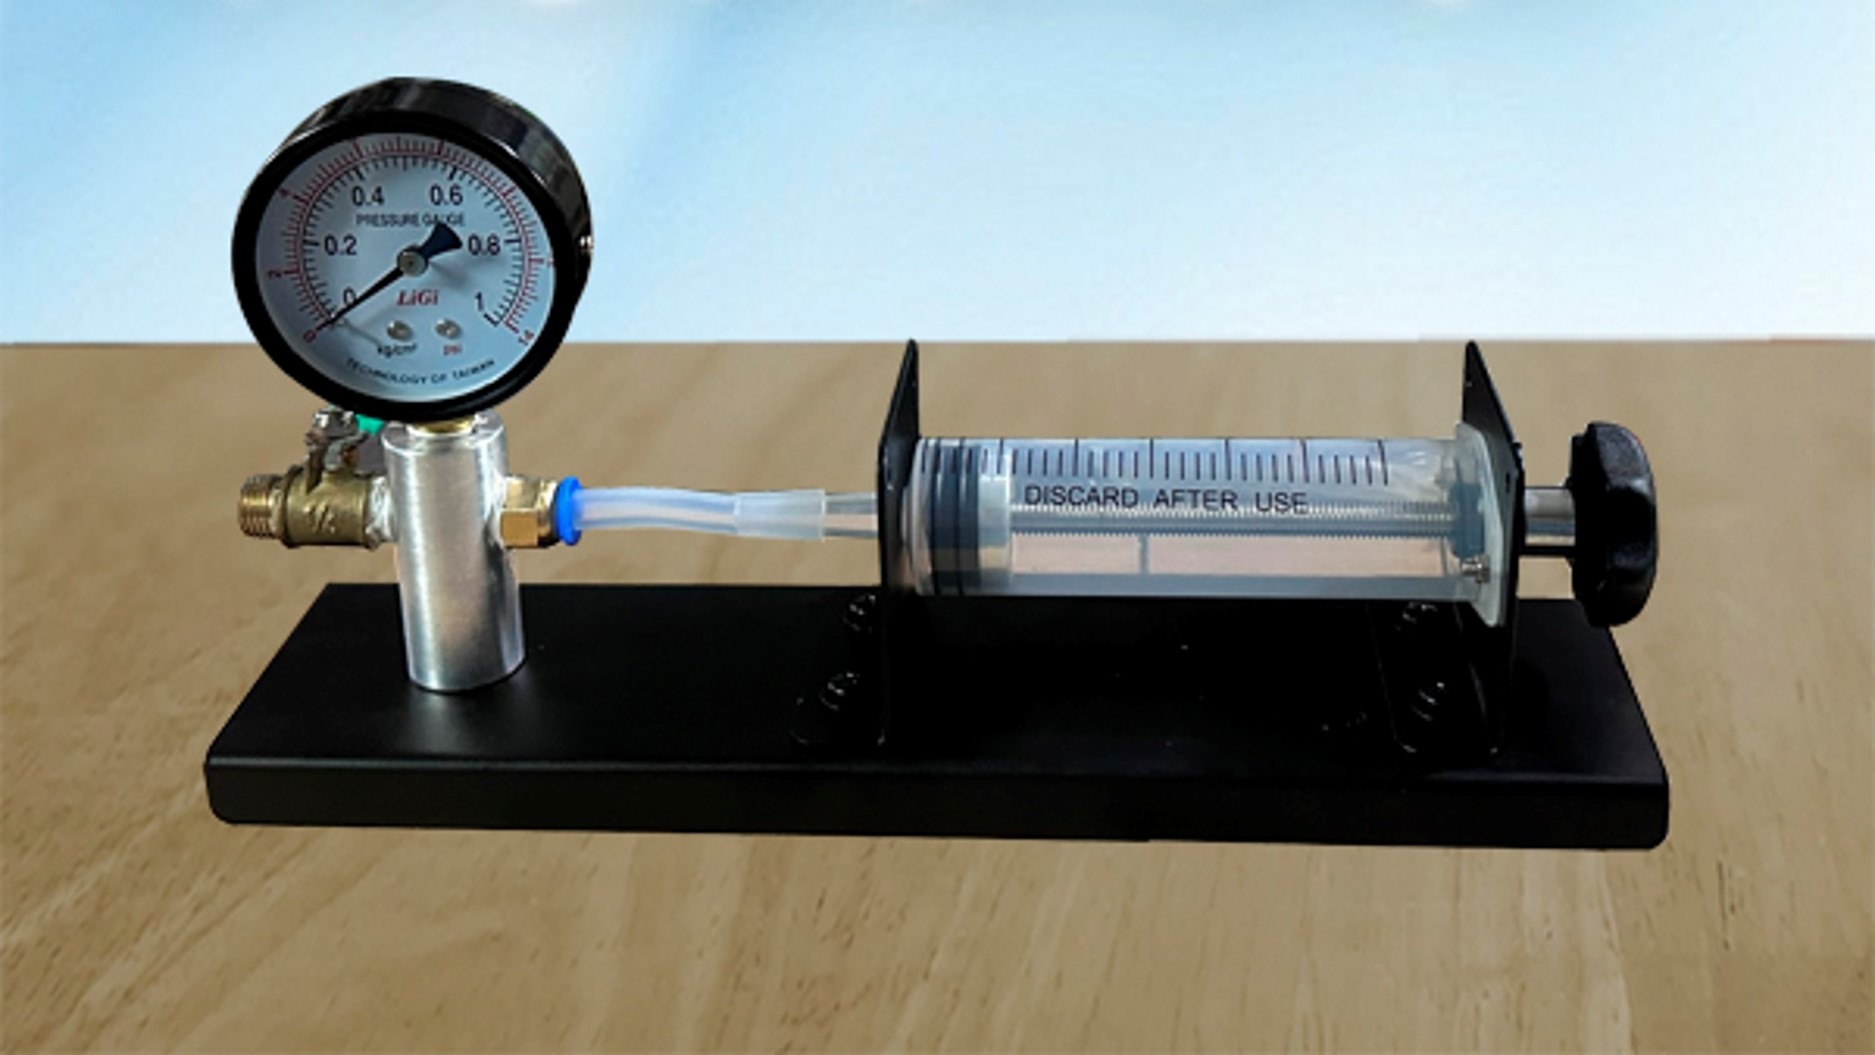
\includegraphics[width=0.3\linewidth]{../figs/D12-2-5}
	\end{center}
	\choice
	{Áp suất không đổi}
	{\True Nhiệt độ không đổi}
	{Thể tích không đổi}
	{Nhiệt độ và áp suất không đổi}
	\loigiai{}
\end{ex}
% ===================================================================
\begin{ex}
	Phát biểu nào sau đây về nội năng là \textbf{không đúng}?
	\choice
	{Nội năng là một dạng năng lượng}
	{Nội năng của một vật có thể tăng hoặc giảm}
	{\True Nội năng là nhiệt lượng}
	{Nội năng có thể chuyển hoá thành các dạng năng lượng khác}
	\loigiai{}
\end{ex}
% ===================================================================
\begin{ex}
	Với cùng một chất, quá trình chuyển thể nào sẽ làm giảm lực tương tác giữa các phân tử nhiều nhất?
	\choice
	{\True Hoá hơi}
	{Đông đặc}
	{Nóng chảy}
	{Ngưng tụ}
	\loigiai{}
\end{ex}
% ===================================================================
\begin{ex}
	Đơn vị nào sau đây không phải là đơn vị đo áp suất?
	\choice
	{$\si{\milli\meter Hg}$}
	{\True $\si{HP}$}
	{$\si{bar}$}
	{$\si{\newton/\meter^2}$}
	\loigiai{}
\end{ex}
% ===================================================================
\begin{ex}
	Nội dung nào dưới đây \textbf{không phải} là sự thể hiện của hiện tượng bay hơi của vật chất?
	\choice
	{Bật quạt sau khi lau sàn nhà}
	{\True Xuất hiện các giọt nước ở thành ngoài cốc nước giải khát có đá khi để trong không khí}
	{Sử dụng khí gas ($\ce{R}-32$) trong các thiết bị làm lạnh của máy điều hoà không khí}
	{Sản xuất muối của các diêm dân}
	\loigiai{}
\end{ex}
% ===================================================================
\begin{ex}
	Khi đi tham quan trên các vùng núi cao có nhiệt độ thấp hơn nhiều dưới đồng bằng, chúng ta cần mang theo áo ấm để sử dụng vì
	\choice
	{mặc áo ấm để ngăn hơi lạnh truyền vào trong cơ thể}
	{mặc áo ấm để ngăn nhiệt độ cơ thể truyền ra ngoài môi truờng}
	{\True mặc áo ấm để ngăn cơ thể mất nhiệt lượng quá nhanh}
	{mặc áo ấm để ngăn tia cực tím từ Mặt Trời}
	\loigiai{}
\end{ex}
% ===================================================================
\begin{ex}
	Chuyển động nào sau đây không được coi là chuyển động Brown?
	\choice
	{Chuyển động của các hạt bụi lơ lửng trong không khí khi quan sát dưới ánh nắng mặt trời vào buổi sáng}
	{Chuyển động của hạt phấn hoa trong nước}
	{Chuyển động của các hạt mực khi nhỏ các giọt mực vào nước}
	{\True Chuyển động thành dòng của các hạt bụi nhỏ trong ống khói của nhà máy xi măng đang vận hành}
	\loigiai{}
\end{ex}
\Closesolutionfile{ans}
\section{Câu trắc nghiệm đúng/sai} 
\textit{Thí sinh trả lời từ câu 1 đến câu 4. Trong mỗi ý \textbf{a)}, \textbf{b)}, \textbf{c)}, \textbf{d)} ở mỗi câu, thí sinh chọn đúng hoặc sai}
\setcounter{ex}{0}
\Opensolutionfile{ans}[ans/G12-3-TF]
% ===================================================================
\begin{ex}
	\immini{Một mô hình áp kế khí ở hình bên gồm một bình cầu thuỷ tinh có thể tích $\SI{270}{\centi\meter^3}$ gắn với một ống nhỏ AB nằm ngang có tiết diện $\SI{0.1}{\centi\meter^2}$. Trong ống có một giọt thuỷ ngân. Ở $\SI{0}{\celsius}$ giọt thuỷ ngân cách A $\SI{30}{\centi\meter}$. }
	{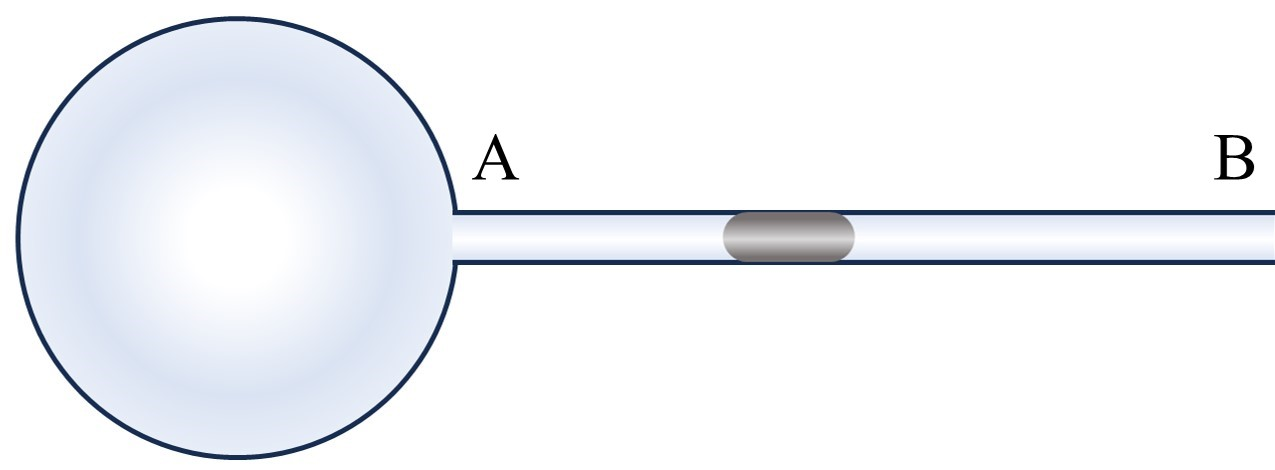
\includegraphics[width=0.5\linewidth]{../figs/D12-2-6}
		
	}
	Sau đó người ta hơ nóng bình cầu để	giọt thủy ngân dịch chuyển đến vị trí mới. Coi thể tích bình là không đổi, ống AB đủ dài để giọt thủy ngân không chảy ra ngoài, khí trong bình là khí lí tưởng.
	\choiceTF[t]
	{\True Áp kế là thiết bị dùng để đo áp suất}
	{Quá trình biến đổi trạng thái của khí trong bình là quá trình đẳng tích}
	{\True Quá trình biến đổi trạng thái của khí trong bình là quá trình đẳng áp}
	{Khi hơ nóng bình cầu đến $\SI{11}{\celsius}$ thì khoảng di chuyển của giọt thuỷ ngân là $\SI{140}{\centi\meter}$}
	\loigiai{
		\begin{itemchoice}
			\itemch Đúng.
			\itemch Sai. Quá trình biến đổi trạng thái của khí trong bình là quá trình đẳng áp.
			\itemch Đúng.
			\itemch Sai. $\dfrac{V_1}{T_1}=\dfrac{V_2}{T_2}\Leftrightarrow \dfrac{270+0,1\cdot30}{273}=\dfrac{270+0,1\cdot\left(30+x\right)}{284}\Rightarrow x=\SI{110}{\centi\meter}.$
		\end{itemchoice}
	}
\end{ex}
% ===================================================================
\begin{ex}
	\immini{Một trong những bệnh nghề nghiệp của thợ lặn có tỉ lệ gây tử vong và mất sức lao động cao là bệnh giảm áp. Nếu một thợ lặn từ độ sâu $\SI{30}{\meter}$ nổi lên mặt nước quá nhanh, nitrogen không vận chuyển kịp đến phổi giải phóng ra ngoài sẽ tích lại trong cơ thể hình thành các bọt khí gây nguy hiểm. }
	{
\includegraphics[width=0.55\linewidth]{../figs/D12-2-7}
	}
	Giả sử sự chênh lệch nhiệt độ là không đáng kể. Cho biết khối lượng riêng của nước là $\SI{1000}{\kilogram/\meter^3}$, áp suất khí quyển là $\SI{1.013E5}{\pascal}$. Lấy $g=\SI{9.8}{\meter/\second^2}$.
	\choiceTF[t]
	{\True Khi thợ lặn nổi lên mặt nước quá nhanh, áp suất giảm đột ngột làm các bọt khí nitrogen nở ra, to dần gây tắc mạch chèn ép các tế bào thần kinh gây liệt, tổn thương các cơ quan}
	{Áp suất người thợ lặn phải chịu khi ở độ sâu $\SI{30}{\meter}$ là $\SI{294}{\kilo\pascal}$}
	{\True Khi nổi lên mặt nước áp suất tại mặt nước khi đó bằng áp suất khí quyển $\SI{1.013E5}{\pascal}$}
	{Thể tích của bọt khí nitrogen (coi là khí lí tưởng) khi lên đến mặt nước lớn gấp 2,9 lần thể tích của bọt khí này ở độ sâu $\SI{30}{\meter}$}
	\loigiai{
		\begin{itemchoice}
			\itemch Đúng.
			\itemch Sai. $p_1=p_0+Dgh=\SI{3.953E5}{\pascal}$.
			\itemch Đúng.
			\itemch Sai. $\dfrac{V_2}{V_1}=\dfrac{p_1}{p_2}=\dfrac{p_1}{p_0}=3,9$.
		\end{itemchoice}
	}
\end{ex}
% ===================================================================
\begin{ex}
	Một học sinh pha chế một mẫu trà sữ bằng cách trộn các mẫu chất lỏng với nhau: nước trà đen (mẫu A), nước đường nâu (mẫu B) và sữa tươi (mẫu C). Các mẫu chất lỏng này chỉ trao đổi nhiệt lẫn nhau mà không gây ra các phản ứng hoá học. Bỏ qua sự trao đổi nhiệt với môi trường và bình chứa. Nhiệt độ trước khi trộn của mẫu A , mẫu B và mẫu C lần lượt là $\SI{10}{\celsius}$, $\SI{15}{\celsius}$ và $\SI{20}{\celsius}$. Biết rằng
	\begin{itemize}
		\item Khi trộn mẫu A với mẫu B với nhau thì nhiệt độ cân bằng của hệ là $\SI{13}{\celsius}$.
		\item Khi trộn mẫu B với mẫu C với nhau thì nhiệt độ cân bằng của hệ là $\SI{18}{\celsius}$.
	\end{itemize}
	\choiceTF[t]
	{\True Khi trộn mẫu A với mẫu B với nhau thì sau khi đạt trạng thái cân bằng nhiệt thì nhiệt độ của mẫu B giảm đi $\SI{2}{\kelvin}$}
	{Nhiệt độ cân bằng của hệ khi trộn mẫu A với mẫu C là $\SI{16}{\celsius}$}
	{Nhiệt độ cân bằng của hệ khi trộn cả ba mẫu với nhau là $\SI{15.5}{\celsius}$}
	{\True Nếu học sinh này pha thêm một mẫu sữa tươi nữa vào hỗn hợp ba mẫu ở câu c thì nhiệt độ cân bằng của hệ lúc này là $\SI{17.5}{\celsius}$}
	\loigiai{
		\begin{itemchoice}
			\itemch Đúng.
			\itemch Sai. \\
			Khi trộn mẫu A và mẫu B:
			$$m_{\mathrm{A}}c_{\mathrm{A}}\left(t_{\mathrm{AB}}-t_{\mathrm{A}}\right)+m_{\mathrm{B}}c_{\mathrm{B}}\left(t_{\mathrm{AB}}-t_{\mathrm{B}}\right)=0\Rightarrow m_{\mathrm{A}}c_{\mathrm{A}}=\dfrac{2}{3}m_{\mathrm{B}}c_{\mathrm{B}}.$$
			Tương tự khi trộn mẫu B và mẫu C:
			$$m_{\mathrm{C}}c_{\mathrm{C}}=\dfrac{3}{2}m_{\mathrm{B}}c_{\mathrm{B}}.$$
			Chọn $m_{\mathrm{B}}c_{\mathrm{B}}=1\Rightarrow\begin{cases}
				m_{\mathrm{A}}c_{\mathrm{A}}=\frac{2}{3}\\
				m_{\mathrm{C}}c_{\mathrm{C}}=1,5
			\end{cases}.$
			\itemch Sai. Khi trộn cả 3 mẫu với nhau thì nhiệt độ cân bằng:
			$$t_{\mathrm{cb}}=\dfrac{m_{\mathrm{A}}c_{\mathrm{A}}t_{\mathrm{A}}+m_{\mathrm{B}}c_{\mathrm{B}}t_{\mathrm{B}}+m_{\mathrm{C}}c_{\mathrm{C}}t_{\mathrm{C}}}{m_{\mathrm{A}}c_{\mathrm{A}}+m_{\mathrm{B}}c_{\mathrm{B}}+m_{\mathrm{C}}c_{\mathrm{C}}}\approx\SI{16.3}{\celsius}.$$
			\itemch Đúng. Khi trộn thêm mẫu sữa tươi vào 3 mẫu trên thì nhiệt độ cân bằng:
			$$t'_{\mathrm{cb}}=\dfrac{m_{\mathrm{A}}c_{\mathrm{A}}t_{\mathrm{A}}+m_{\mathrm{B}}c_{\mathrm{B}}t_{\mathrm{B}}+2m_{\mathrm{C}}c_{\mathrm{C}}t_{\mathrm{C}}}{m_{\mathrm{A}}c_{\mathrm{A}}+m_{\mathrm{B}}c_{\mathrm{B}}+2m_{\mathrm{C}}c_{\mathrm{C}}}=\SI{17.5}{\celsius}.$$
		\end{itemchoice}
	}
\end{ex}
% ===================================================================
\begin{ex}
	Cho một lượng khí lí tưởng nhận công để biến đổi từ trạng thái (1) sang trạng thái (2) như đồ thị hình bên. Biết nhiệt độ của khối khí ở trạng thái (1) là $\SI{600}{\kelvin}$.
	\begin{center}
		\begin{tikzpicture}  
			\begin{axis}[  ultra thick,scale=0.5,
				xmin=0,  
				xmax=12,  
				xtick={0,4,10},
				ytick={0,80},
				minor x tick num=1,
				minor y tick num=1,
				ymin=0,  
				ymax=110, 
				samples=300,
				axis lines=center, 
				xlabel=$\xsi{V}{\left(\si{\deci\meter^3}\right)}$, 		ylabel=$\xsi{p}{\left(\si{\kilo\pascal}\right)}$,
				every axis y label/.style={at=(current axis.above origin),anchor=south},  
				every axis x label/.style={at=(current axis.right of origin),anchor=west},  ]
				\coordinate (A) at (axis cs: 10,80);
				\coordinate (B) at (axis cs: 4,80);
				\coordinate (O) at (axis cs: 0,0);
				\draw[dashed, line width=1pt] (axis cs: 4,0)--(B)--(axis cs:0,80);
				\draw[dashed, line width=1pt] (axis cs: 10,0)--(A)--(axis cs:0,80);
				\draw[line width=1.5pt,blue,decoration={markings, mark=at position 0.5 with {\arrow{stealth}}},
				postaction={decorate}] (A)--(B);
				\node[above] at (A) {(1)};
				\node[above] at (B) {(2)};
			\end{axis}  
			\node[below left] at (O) {O};
		\end{tikzpicture}
	\end{center}
	\choiceTF[t]
	{Nhiệt độ của khối khí ở trạng thái (2) là $\SI{240}{\celsius}$}
	{\True Khối khí nhận một công có giá trị $\SI{480}{\joule}$}
	{Khối khí nhận từ môi trường bên ngoài một nhiệt lượng $\SI{1620}{\joule}$}
	{Nội năng của khối khí tăng thêm một lượng $\SI{1140}{\joule}$}
	\loigiai
	{
		\begin{itemchoice}
			\itemch Sai. Đẳng áp: $\dfrac{V_1}{T_1}=\dfrac{V_2}{T_2}\Rightarrow T_2=\SI{240}{\kelvin}$.
			\itemch Đúng. $A=-A'=p\left(V_1-V_2\right)=\SI{480}{\joule}$.
			\itemch Sai. Vì $T_2<T_1$ nên khối khí tỏa nhiệt.
			\itemch Sai. Vì $T_2<T_1$ nên nội năng khí giảm.
		\end{itemchoice}
	}
\end{ex}
\Closesolutionfile{ans}
\section{Câu trắc nghiệm trả lời ngắn} \textit{Thí sinh trả lời từ câu 1 đến câu 6}
\setcounter{ex}{0}
\Opensolutionfile{ans}[ans/G12-3-TL]
% ===============================================================
\begin{ex}
	Đồ thị biểu diễn sự phụ thuộc thể tích $V$ của một khối khí lí tưởng xác định theo nhiệt độ $t$ khi áp suất không đổi có dạng như hình vẽ. Nhiệt độ tại vị trí A bằng bao nhiêu $\si{\celsius}$? \textit{(Kết quả làm tròn đến phần nguyên)}.
	
	\begin{center}
		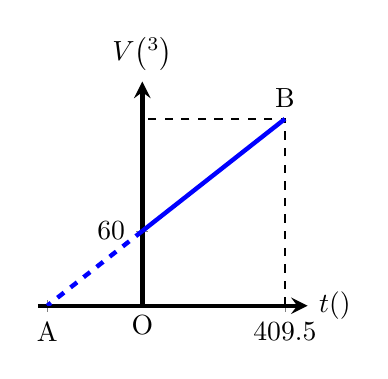
\begin{tikzpicture}  
			\begin{axis}[  ultra thick,scale=0.5,
				xmin=-300,  
				xmax=475,  
				xtick={-273,0,409.5},
				ytick={0,60},
				ymin=0,  
				xticklabels={A,0,409.5},
				ymax=180, 
				samples=300,
				axis lines=center, 
				xlabel=$\xsi{t}{\left(\si{\celsius}\right)}$, 		ylabel=$\xsi{V}{\left(\si{\centi\meter^3}\right)}$,
				every axis y label/.style={at=(current axis.above origin),anchor=south},  
				every axis x label/.style={at=(current axis.right of origin),anchor=west},  
				]
				\draw[dashed, line width=1pt] (axis cs: 409.5,0)--(axis cs: 409.5,150)--(axis cs: 0,150);
				\addplot [ultra thick, blue, smooth, domain=0:409.5] {60+20*x/91} ; 
				\addplot [ultra thick, blue, dashed,smooth, domain=0:-273] {60+20*x/91} ; 
				\node[above] at (409.5,150) {B};
				\coordinate (O) at (axis cs: 0,0);
			\end{axis}
			\node[below] at (O) {O};  
		\end{tikzpicture}
	\end{center}
	\shortans{ -273}
	\loigiai{
		Đẳng áp nên $\dfrac{V_{\mathrm{B}}}{T_{\mathrm{B}}}=\dfrac{V_{\mathrm{O}}}{T_{\mathrm{O}}}\Rightarrow V_{\mathrm{B}}=\SI{150}{\centi\meter^3}$.\\
		Ta có $V$ là hàm tuyến tính theo $t$ nên:
		$$\dfrac{t_{\mathrm{A}}-t_{\mathrm{O}}}{t_{\mathrm{B}}-t_{\mathrm{O}}}=\dfrac{V_{\mathrm{A}}-V_{\mathrm{O}}}{V_{\mathrm{B}}-V_{\mathrm{O}}}\Rightarrow t_{\mathrm{A}}=\SI{-273}{\celsius}.$$
	}
\end{ex}
% ===============================================================
\begin{ex}
	Biết nhiệt nóng chảy riêng của nước đá là $\SI{3.4E5}{\joule/\kilogram}$. Nhiệt lượng cần cung cấp để làm nóng chảy hoàn toàn $\SI{50}{\gram}$ nước đá ở $\SI{0}{\celsius}$ bằng bao nhiêu $\si{\kilo\joule}$? \textit{(Kết quả làm tròn đến phần nguyên)}.
	\shortans{ 17}
	\loigiai{
		$$Q=m\lambda=\SI{17}{\kilo\joule}.$$
	}
\end{ex}
% ===============================================================
\begin{ex}
	\immini{
		Một học sinh Trường TH - THCS - THPT Lê Thánh Tông làm thí nghiệm đun nóng chất X trên bếp điện và vẽ được đồ thị biểu diễn sự phụ thuộc nhiệt độ $\xsi{T}{(\celsius})$ của nó theo thời gian $\xsi{t}{(\minute)}$ như hình bên. Giá trị mỗi ô theo trục hoành là 5 phút, theo trục tung là $\SI{25}{\celsius}$. Trong quá trình thí nghiệm, chất X tan chảy và sau một thời gian nó sôi lên. Do vội vàng, học sinh này quên ghi nhiệt độ ban đầu của chất đó mà chỉ nhớ rằng trong 15 phút đầu công suất đốt nóng của bếp kém hơn 2 lần so với thời gian còn lại. Giả sử rằng năng lượng nhiệt tỏa ra từ bếp điện chỉ dùng để đun nóng chất X. Gọi nhiệt dung của chất X ở trạng thái rắn là $C_{1}$ và ở trạng thái lỏng là $C_{2}$. 
	}
	{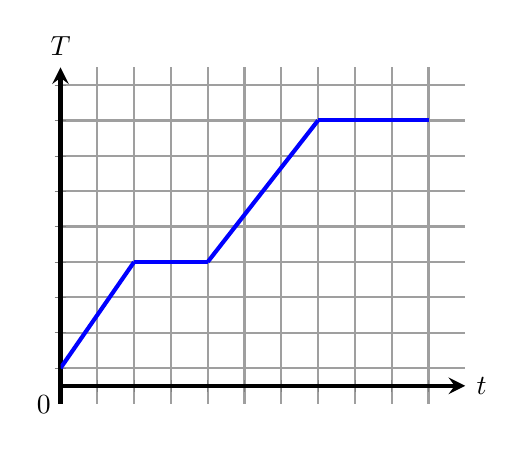
\begin{tikzpicture}  
			\begin{axis}[  ultra thick,scale=0.75,
				xmin=0,  
				xmax=11,  
				xtick={0,1,...,10},
				ytick={0,0.5,1.5, 2.5, 3.5,...,8.5},
				minor x tick num=0,
				minor y tick num=0,
				ymin=-0.5,  
				ymax=9, 
				samples=300,
				yticklabels=\empty,
				xticklabels=\empty,
				yticklabel style={/pgf/number format/.cd, fixed,
					fixed zerofill, precision=1}, %số chữ số thập phân
				axis lines=center, 
				grid style={step=1, line width =0.4pt, color=gray!40!white},
				grid=both, %giới hạn ô lưới
				major grid style={line width=0.8pt,gray!75!white},
				xlabel=$t$, 		ylabel=$T$,
				every axis y label/.style={at=(current axis.above origin),anchor=south},  
				every axis x label/.style={at=(current axis.right of origin),anchor=west},  ]
				\coordinate (O) at (0,0);
				\addplot [line width=1.5pt, blue, smooth, domain=0:2] {0.5+1.5*x};  
				\addplot [line width=1.5pt, blue, smooth, domain=2:4] {3.5};  
				\addplot [line width=1.5pt, blue, smooth, domain=4:7] {3.5+4*(x-4)/3};  
				\addplot [line width=1.5pt, blue, smooth, domain=7:10] {7.5};   
			\end{axis}  
			\node[below left]at (O) {0};
		\end{tikzpicture}
		
	}
	Tỉ số $C_{2} / C_{1}$ bằng bao nhiêu? \textit{(Kết quả lấy đến hai chữ số sau dấu phẩy thập phân)}.
	\shortans{2,25 }
	\loigiai{
		\begin{equation}
			\calP_1t_1=mC_1\Delta t_1\Leftrightarrow \calP_1\cdot 10=mC_1 \cdot25\cdot3
			\label{eq:1}
		\end{equation}
		\begin{equation}
			\calP_2t_2=mC_2\Delta t_2\Leftrightarrow 2\calP_1\cdot 15=mC_2 \cdot25\cdot4
			\label{eq:2}
		\end{equation}
		Từ \eqref{eq:1} và \eqref{eq:2}:
		$$\dfrac{C_2}{C_1}=\dfrac{30}{10}\cdot\dfrac{3}{4}=2,25.$$	}
\end{ex}
% ===============================================================
\begin{ex}
	\immini{
		Chuông lặn là một thiết bị chìm dưới nước để nghiên cứu các điều kiện trong nước, cũng có thể được sử dụng làm thiết bị lặn để sửa chữa các bộ phận dưới nước của trụ cầu và các công trình xây dựng khác. Một chuông lặn cao $\SI{2}{\meter}$ được thả chìm theo phương thẳng đứng từ mặt nước xuống đáy hồ nước sâu $\SI{10}{\meter}$ (hình vẽ). }	
	{
		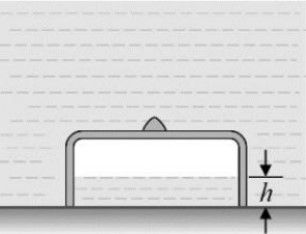
\includegraphics[width=0.45\linewidth]{../figs/D12-2-8}
	}
	Giả sử nhiệt độ của khối khí (coi là khí lí tưởng) kèm theo trong chuông không đổi, áp suất khí quyển $p_{0}=\SI{E5}{\pascal}$, khối lượng riêng của nước là $\rho=\SI{E3}{\kilogram/\meter^3}$ và lấy $g=\SI{10}{\meter/\second^2}$. Độ cao $h$ của mực nước trong chuông bằng bao nhiêu mét? \textit{(Kết quả lấy đến hai chữ số sau dấu phẩy thập phân)}
	\shortans{0,95}
	\loigiai{
		\begin{center}
			\begin{tabular}{|M{5cm}|M{5cm}|M{5cm}|}
				\hline
				& $p$ &$V$\\
				\hline
				\thead{Ban đầu}&$p_0=\SI{E5}{\pascal}$ & $V_0=2S$\\
				\hline
				\thead{Lúc sau} & $p=p_0+\rho g\left(H-h\right)=10^5+10^4\cdot\left(10-h\right)$ & $V=\left(2-h\right)S$\\
				\hline
			\end{tabular}
		\end{center}
		Áp dụng định luật Boyle:
		$$p_0V_0=pV\Leftrightarrow 10^5\cdot2S=\left[10^5+10^4\cdot\left(10-h\right)\right]\cdot\left(2-h\right)S\Rightarrow h\approx\SI{0.95}{\meter}.$$
	}
\end{ex}
% ===============================================================
\begin{ex}
	\immini{
		Một khối khí lí tưởng thực hiện một chu trình biến đổi như hình vẽ. Cho $p$ là áp suất và $V$ là thể tích của khối khí. Biết $1-2$ là quá trình đẳng tích và $2-3$ là quá trình đẳng áp. Nhiệt độ của khối khí ở trạng thái 1 và 3 lần lượt là $T_{1}=\SI{320}{\kelvin}$ và $T_{3}=\SI{480}{\kelvin}$. Nhiệt độ của khối khí ở trạng thái 2 bằng bao nhiêu theo thang Kelvin $\left(\si{\kelvin}\right)$? \textit{(Kết quả làm tròn đến phần nguyên)}.
	}
	{
		\begin{tikzpicture}  
			\begin{axis}[  ultra thick,scale=0.5,
				xmin=0,  
				xmax=7,  
				ymin=0,  
				ymax=8, 
				samples=300,
				xtick=\empty,
				ytick=\empty,
				yticklabels=\empty,
				xticklabels=\empty,
				axis lines=center, 
				xlabel=$V$, 		ylabel=$p$,
				every axis y label/.style={at=(current axis.above origin),anchor=south},  
				every axis x label/.style={at=(current axis.right of origin),anchor=west},  ]
				\coordinate (A) at (axis cs: 2,2);
				\coordinate (B) at (axis cs: 2,6);
				\coordinate (C) at (axis cs: 6,6);
				\coordinate (O) at (axis cs: 0,0);
				\draw[blue, line width=1.5pt, decoration={markings, mark=at position 0.5 with {\arrow{stealth}}},
				postaction={decorate}] (A)--(B);
				\draw[blue, line width=1.5pt, decoration={markings, mark=at position 0.5 with {\arrow{stealth}}},
				postaction={decorate}] (B)--(C);
				\draw[blue, line width=1.5pt, decoration={markings, mark=at position 0.5 with {\arrow{stealth}}},
				postaction={decorate}] (C)--(A);
				\draw[line width=1pt, dashed] (O)--(A);
				\node[left] at (A) {(1)};
				\node[above left] at (B) {(2)};
				\node[above] at (C) {(3)};
			\end{axis}  
			\node[below left] at(O) {0};
		\end{tikzpicture}
	}
	\shortans{392 }
	\loigiai{
		Ta có:
		$$\begin{cases}
			\dfrac{p_2}{p_1}=\dfrac{T_2}{T_1}\\
			\dfrac{V_3}{V_2}=\dfrac{T_3}{T_2}
		\end{cases}\ \text{hay} \ \begin{cases}
			\dfrac{p_3}{p_1}=\dfrac{T_2}{T_1}\\
			\dfrac{V_3}{V_1}=\dfrac{T_3}{T_2}
		\end{cases}$$
		Mà đường thẳng $(3)\rightarrow(1)$ đi qua gốc tọa độ nên:
		$$\dfrac{p_3}{p_1}=\dfrac{V_3}{V_1}\Rightarrow \dfrac{T_2}{T_1}=\dfrac{T_3}{T_2}\Rightarrow T_2=\sqrt{T_3T_1}\approx\SI{392}{\kelvin}.$$
	}
\end{ex}
% ===============================================================
\begin{ex}
	\immini{
		Một bạn học sinh đã thiết kế một thiết bị thí nghiệm để đo nhiệt độ môi trường bằng cân điện tử như hình bên. Xilanh dẫn nhiệt có đầu trên hở và được cố định trên bàn. Một pit-tông có khối lượng $m_{1}=\SI{600}{\gram}$ và diện tích mặt cắt ngang $S=\SI{20}{\centi\meter^2}$ được dùng để bịt kín một khối lượng khí lí tưởng nhất định trong xilanh. Bỏ qua ma sát giữa pit-tông và thành xilanh. 
	}
	{
		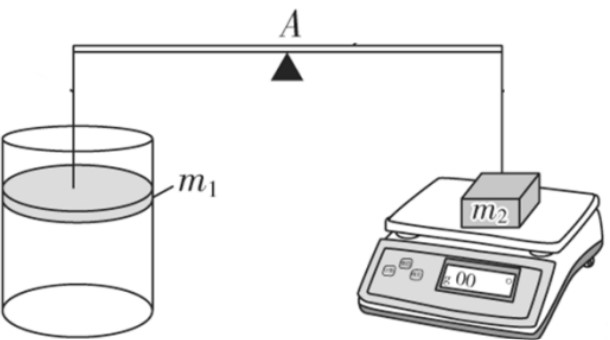
\includegraphics[width=0.55\linewidth]{../figs/D12-2-9}
	}
	Trọng tâm (điểm chính giữa) của một thanh nhẹ được đặt trên điểm tựa cố định A. Pit-tông được treo thẳng đứng ở đầu bên trái của thanh bằng một sợi dây nhẹ, không dãn. Một khối sắt có khối lượng $m_{2}=\SI{1200}{\gram}$ được treo thẳng đứng ở đầu bên phải bằng một sợi dây nhẹ, không dãn; khối sắt được đặt lên cân điện tử. Khi cân điện tử hiển thị giá trị ổn định 600 g thì nhiệt độ môi trường đo được là $\SI{27}{\celsius}$. 
	Cho áp suất khí quyển $p_{0}=\SI{E5}{\pascal}$ và lấy $g=\SI{10}{\meter/\second^2}$. Nhiệt độ lớn nhất mà thiết bị thí nghiệm này có thể đo được bằng bao nhiêu $\si{\celsius}$? \textit{(Kết quả làm tròn đến phần nguyên)}.
	\shortans{36 }
	\loigiai{
		Nếu nhiệt độ khí trong xilanh tăng, áp suất khí tăng, pit-tông bị đẩy đi lên $\Rightarrow$ dây bị chùn, thí nghiệm không còn đo được.\\
		\begin{center}
			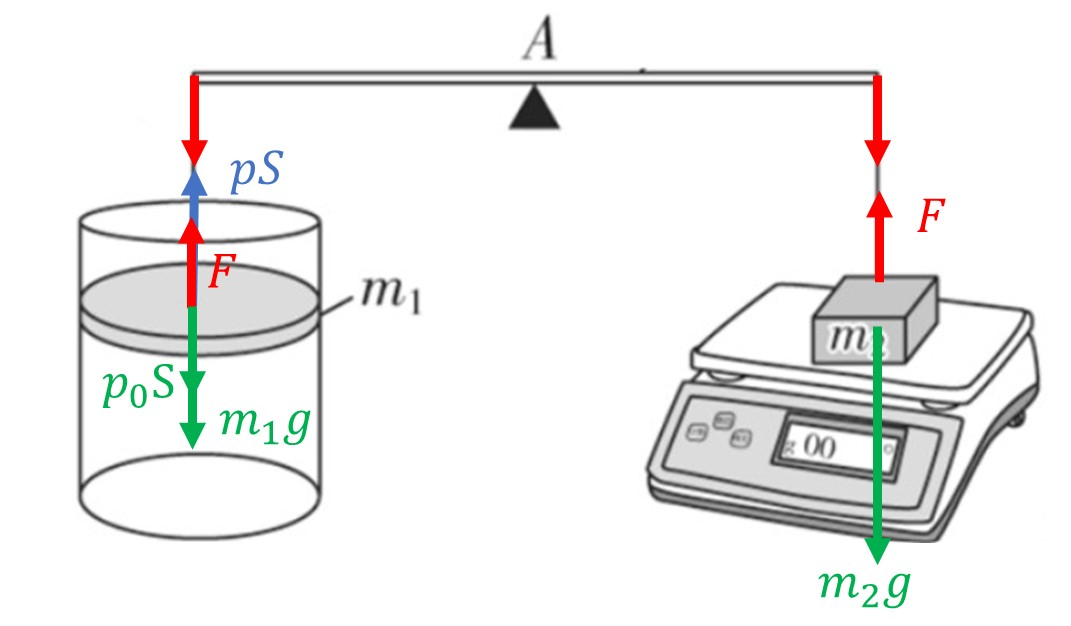
\includegraphics[width=0.5\linewidth]{../figs/D12-2-10}
		\end{center}
		Vật nặng $m_2$ cân bằng:
		$$m_2g-F=mg\Rightarrow F=\left(m_2-m\right)g.$$
		Pit-tông cân bằng:
		$$pS+F=m_1g+p_0S\Rightarrow p=\dfrac{m_1g+p_0S-F}{S}=\dfrac{\left(m_1+m-m_2\right)g+p_0S}{S}.$$
		Tại nhiệt độ $T_1=\SI{300}{\kelvin}$ thì số chỉ của cân là $m=\SI{600}{\gram}$, khi đó áp suất khí trong xilanh là:
		$$p_1=p_0=\SI{E5}{\pascal}.$$
		Thí nghiệm sẽ không còn đo được khi dây chùn $\left(F=0\right)$, khi đó:
		$$p_2=\dfrac{m_1g+p_0S}{S}=\SI{1.03E5}{\pascal}.$$
		Trong quá trình thí nghiệm, dây không chùn nên thể tích khí trong xilanh không đổi:
		$$\dfrac{p_2}{T_2}=\dfrac{p_1}{T_1}\Rightarrow T_2=\SI{309}{\kelvin}\Rightarrow t_2=\SI{36}{\celsius}.$$
	}
\end{ex}
\Closesolutionfile{ans}
\begin{center}
	\textbf{-- HẾT --}
\end{center}